% Section Delegation Mapping:
%
% --------------------> Brady
% Introduction
% Overview
% --------------------
%
% Hardware
%   -FPGA Board ----------------> Nate
%   -Breakout Box --------------> Isabella
%   -FSS PCB -------------------> Jacob
%   -FSS Housing ---------------> Brady & Isabella
%
% CR16 Processor --------------->Nate
%
% --------------------> Jacob
% Peripheral Interfacing
% Assembler
% --------------------
%
% Firmware --------------------> Jacob & Nate
% Lessons Learned -------------> Everyone
%
% --------------------> Isabella
% About the Team
% Conclusion and Future Work
% --------------------

\documentclass[conference]{IEEEtran}
\usepackage{amsmath,amssymb,amsfonts}
\usepackage{algorithmic}
\usepackage{graphicx}
\usepackage{geometry}
\usepackage{textcomp}
\usepackage{xcolor}
\usepackage{array}
\usepackage{ragged2e}
\usepackage{multirow} % For multirows in tables
\usepackage{float} % Appending the [H] option forces the placement of a figure in the place it's in the code
\usepackage[numbers]{natbib} % For integration with bibliography commands
\usepackage{pdfpages}
\usepackage{hyperref}
\usepackage{chngpage}
\usepackage[utf8]{inputenc}
\usepackage{listings}

\usepackage{xparse}
\NewDocumentCommand{\code}{v}{%
\texttt{\textcolor{black}{#1}}%
}

\hypersetup{
    colorlinks=true,
    linkcolor=blue,
    filecolor=magenta,
    urlcolor=cyan,
    citecolor=magenta
}

\def\BibTeX{{\rm B\kern-.05em{\sc i\kern-.025em b}\kern-.08em
    T\kern-.1667em\lower.7ex\hbox{E}\kern-.125emX}}

\geometry{
    a4paper,
    left=0.5in,
    top=0.5in,
    right=0.5in,
    bottom=0.5in
}

\begin{document}

\begin{titlepage}
\begin{adjustwidth}{+1in}{+1in}
\begin{center}
    \vspace*{6.5cm}
    \Huge
    \textbf{Final Report: The Fully-Synchronized Synthesizer (FSS) Interface Prototype}

    \vspace{1cm}
    \LARGE
    Computer Design Laboratory ECE 3710\\
    Fall 2021\\
    The University of Utah

    \vspace{1cm}

    \normalsize
    \centering
    \begin{adjustwidth}{-1.5in}{-1.5in} % Adjust the L and R margins by 1 inch
    \begin{center}
        \begin{tabular}{ c c c c }
        \centering
        Jacob Peterson & Brady Hartog & Isabella Gilman & Nate Hansen\\
        \textit{Computer Engineering 2022} & \textit{Computer Engineering 2022} & \textit{Computer Engineering 2023} & \textit{Computer Engineering 2023}\\
        \textit{University of Utah} & \textit{University of Utah} & \textit{University of Utah} & \textit{University of Utah}\\
        Salt Lake City, UT & Salt Lake City, UT & Salt Lake City, UT & Salt Lake City, UT\\
        \end{tabular}
    \end{center}
    \end{adjustwidth}
\end{center}
\end{adjustwidth}
\end{titlepage}

\begin{abstract}
We present the design and implementation of a small-scale prototype for a fully-synchronized synthesizer (“FSS”) interface. The prototype is designed to address a major drawback of contemporary musical synthesizers. As a proof of concept for an innovative user interface, the prototype casts a vision for a more versatile and powerful synthesizer for the musical artists of tomorrow. Pursuant to the course objectives of ECE 3710, the principal component of the prototype is an Intel Cyclone V FPGA. This report chronicles our process of programming and interfacing with the FPGA as well as crafting a hardware system to deliver a prototype with a highly intentional and interactive user experience.
\end{abstract}

\begin{figure*}[bhtp]
    \centering
    \includegraphics[scale=0.6]{./resources/figures/full_assembly_block_diagram.jpg}
    \caption{High level block diagram of the full FSS hardware assembly.}
    \label{fig:full_fss_block_diagram}
\end{figure*}

\section{Introduction}

In 1978 the music technology firm Sequential Circuits introduced the Prophet-5 musical synthesizer. Prophet-5 was among the world’s first \textit{fully-programmable} synthesizers, meaning that every controllable parameter could be stored in user-defined programs. Full programmability was a major milestone in the history of the synthesizer, and Prophet-5 would set the precedent of synthesizer design for decades to come.

In fact, over 40 years later, Prophet-5 remains the archetype of modern hardware synthesizers. Whereas the fully-programmable paradigm of Prophet-5 is highly useful, it suffers a major drawback. Fig. \ref{fig:param_analog} illustrates the drawback. In the fully-programmable paradigm, each parameter has both a \textit{physical value} and an \textit{active value}. The physical value is the value indicated by the position of the dial. The active value is set either by: 1) changing the position of the dial (in which case it is the same as the physical value); or by 2) recalling a user-defined program. Naturally, recalled values do not necessarily match—and in practice seldom do match—the physical values of the dials. We say that parameters controlled in this way are \textit{unsynchronized}.

\begin{figure}[h]
    \centering
    \includegraphics[scale=0.27]{./resources/figures/param_analog.png}
    \caption{The drawback with traditional, analog level meters. The physical and active values are out of sync!}
    \label{fig:param_analog}
\end{figure}

The drawback described above assumes the use of traditional, analog level meters as shown in Fig. \ref{fig:param_analog}. Fig. \ref{fig:param_digital} depicts a proposed alternative to the traditional level meter. This level meter consists of an LED ring display with digital control. By leveraging digital control, the level meter can display the active value of the parameter at all times, whether it is set by changing the dial or by recalling a program. We say that a parameter controlled in this way is \textit{synchronized}.

\begin{figure}[h]
    \centering
    \includegraphics[scale=0.27]{./resources/figures/param_digital.png}
    \caption{The proposed digital level meter to implement synchronized parameters.}
    \label{fig:param_digital}
\end{figure}

We envision a musical synthesizer for which every parameter on the control panel is synchronized; such would be a \textit{fully-synchronized} synthesizer (``FSS'').

In this report we present the design and implementation of a small-scale prototype for an FSS interface (Fig. \ref{fig:fss_cover_art}) with respect to the learning objectives of ECE 3710. We believe our prototype is a successful proof of concept for the FSS interface as well as a clear, articulate and creative application of our computer engineering skills to date. We hope you enjoy our presentation of the FSS interface prototype.

\begin{figure}[h]
    \centering
    \includegraphics[scale=0.27]{./resources/figures/fss_cover_art.png}
    \caption{The FSS prototype.}
    \label{fig:fss_cover_art}
\end{figure}

\section{Overview}

The following is an overview of the user-facing functionality of the FSS prototype.

The FSS prototype has three synchronized parameters and three user-defined programs. The objective of the device is to demonstrate that all three parameters can be stored in each of the programs and recalled on demand.

Turning any of the parameter dials will change the value in its ring display by a corresponding amount. As soon as any parameter is changed beyond the programmed state, the save button LED turns on. The user may save their changes by pressing the save button, whereupon the save button LED turns off. The user may recall programs by pressing the corresponding program buttons.

The play/pause button is intended for auxiliary functionality, such as playing a sound if the FSS prototype is connected to an audio engine. In our implementation, the play/pause button is used to trigger animations of the display elements for aesthetic purposes.

\section{Hardware}
The hardware assembly of our device consists of 3 main components: A DE1-SoC Cyclone V FPGA board, a small breakout box for power supply and I$^2$C bus interfacing, and our FSS Prototype device. These components and their connections can be seen at a high level in Fig. \ref{fig:full_fss_block_diagram}.

\subsection{FPGA Board}
The FPGA device drives all of the logical control for the FSS device. This is accomplished by instantiating a single module of our CR16 processor, and adding to that a set of peripheral modules. The modules that are peripheral to CR16 are responsible for allowing the assembly code access to important device data such as the state of the buttons and rotary encoders, the state of the LED indicators, and a 48-bit microsecond counter for I$^2$C timing. All of these modules were coded in SystemVerilog HDL and are available within the GitHub repository ``FSSPrototype''. The FPGA acts as an I$^2$C master, where GPIO pins 1 and 2 are the SCL and SDA lines respectively, as shown in Fig. \ref{fig:gpio_mapping} The FPGA is also attached to a common ground shared by the FSS Prototype device and the breakout box. In order for the device to function, the FPGA must be successfully programmed with the \code{fss_top.v} top-level Verilog module, and that module must include the \code{fss.dat} machine code file.

\begin{figure*}[bhtp]
    \centering
    \includegraphics[scale=0.5]{./resources/figures/gpio_pin_map.jpg}
    \caption{GPIO pin diagram as obtained from the Cyclone V user manual with mappings added \cite{cite:de1-soc_manual}.}
    \label{fig:gpio_mapping}
\end{figure*}

The FPGA device allowed our team to employ a variety of useful testing methods, such as displaying data from BRAM on the bank of seven-segment displays, assigning an FPGA button to a global reset, and testing I$^2$C communication. Our device relies on the 50MHz clock housed on the FPGA, but we could also slow down execution during debugging by tying the clock signal to a button. Successful design and testing of this project relied on substantial interfacing with the FPGA.

\subsection{Breakout Box}
The breakout box is responsible for powering the FSS prototype interface as well as forwarding the I$^2$C signal coming from the FPGA to the port expander on the main PCB. The housing of the breakout box contains a USB type-A receptacle, a USB type-B receptacle, 2 male pin headers, a buck converter, and a rocker switch. The USB type-B receptacle is responsible for receiving power from the USB cable voltage bus and delivering it to the breakout PCB and then the main PCB. This power cable supplies 5V to the board from a DC power source, which is generally a wall adapter plugged into a standard outlet. From here the voltage is stepped down to 3.3V by a DC-DC buck converter contained within the breakout box to ensure the main PCB is receiving the correct voltage. Then, the USB type-A cable supplies this power to the main PCB board. To make control of power simple, the breakout box also includes a rocker switch that toggles power on and off.

The control logic sent by the FPGA is also routed through the breakout box. The FPGA drives the I$^2$C bus lines, both SDA (serial data) and SCL (serial clock), using the GPIO pin headers on the FPGA board with an open-drain configuration. Breadboard wires then connect the two bus lines from the FPGA board to the breakout box, and the breakout PCB routes the two bus lines to the USB type-A cable which is then connected to the FSS prototype. The USB type-A cable's D+ and D- differential data pins are adapted to be the SCL and SDA signals of the I$^2$C bus respectively.

The breakout box schematic and PCB layout are shown in Figures \ref{fig:breakout_schematic} and \ref{fig:breakout_pcb} respectively.

\begin{figure*}[bhtp]
    \centering
    \includegraphics[width=4.5in]{./resources/figures/breakout_schematic.pdf}
    \caption{Schematic of Breakout PCB.}
    \label{fig:breakout_schematic}
\end{figure*}

\begin{figure*}[bhtp]
    \centering
    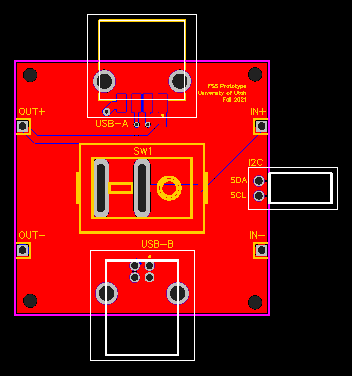
\includegraphics[width=4in]{./resources/figures/breakout_pcb.pdf}
    \caption{Layout of Breakout PCB.}
    \label{fig:breakout_pcb}
\end{figure*}

\subsection{FSS PCB}
The FSS Prototype's PCB is responsible for all the electronic circuitry on the device. In this document, we refer to this PCB as the ``main'' PCB and it resides within the prototype's housing. We wanted to preserve the beauty factor of our FSS prototype, so instead of using many breadboard wires to interface the main PCB to the FPGA board, we opted to use a single USB cable that is inserted into the back of the prototype's housing. A USB Mini type-B receptacle connects this USB cable from the breakout box to the main board, and is used to provide power throughout the board and, as mentioned previously, adapts the D+ and D- differential data pins as the SCL and SDA signals of the I$^2$C bus. All communication from the FPGA to the main board must take place serially since it's impractical to drive the board's components individually using the PMOD pin headers on the FPGA board. So, to drive the board's components serially, the \code{GMSB0522102Y7EU} 8-bit I/O port expander IC is used. Two of these port expander chips in conjunction provide complete I/O to the entirety of the main PCB and the serial communication protocol to interface with them is I$^2$C in standard mode ($100$ kHz clock speed). This port expander chip is quasi-bidirectional, meaning that there is no configuration register to specify whether a port is an input or an output. Instead, to use a port as an input, the port is driven high and can be pulled low by an external component. 5 tactile push buttons with a pull-up configuration are connected to one of the I/O port expander chips. Additionally, there are 3 quadrature-encoded, mechanical rotary encoders each with two channels --- A and B. The individual channels use a pull-up configuration and are connected to one of the I/O port expander chips. These two channels in conjunction make up the quadrature-encoded output of these rotary encoders.

The FSS Prototype contains 62 LEDs with an amber hue. There are 19 LEDs in each of the 3 ring displays and 1 LED for each of the 5 button indicator lights. To drive all of these LEDs using minimal I/O, 4 of the \code{STP16CPC05MTR} 16-bit, latching, shift-register LED driver ICs are used. Each driver contains the following pins: \code{SDI} (serial data in) which the input to the shift register, \code{SDO} (serial data out) which contains the bit shifted out of the shift register, \code{CLK} (clock) which synchronizes \code{SDI} and \code{SDO}, \code{LE} (latch enable) which latches the driver output when asserted, \code{OE} (output enable) which is the active-low enable pin, and \code{R-EXT} which controls the chip's internal current limiter to provide a constant-current source to the LEDs. These 4 LED driver ICs on the main board are daisy-chained together and the first driver in the chain has its \code{SDI} pin connected to one of the ports on the I/O port expander chip. Additionally, one of the I/O port expander chips drives all 4 \code{CLK} and \code{LE} signals of the LED drivers so that they are all synchronized.

The SDA and SCL lines of the I$^2$C bus are short-circuit protected using $300 \Omega$ series resistors. This resistance is low enough that it does not affect the I$^2$C bus capacitance, which is limited to $400$ picofarads in standard mode. Additionally, the 6 ft. braided USB cable used to interface with the main board is shielded, has a low resistance, and a low capacitance, so the I$^2$C bus timing requirements are met without an issue. As part of the I$^2$C specification, the SDA and SCL lines are directly connected to 3.3V using two $2 \text{k}\Omega$ pull-up resistors.

As another precaution, series resistors are used to protect against accidental short-circuits on the pull-up/pull-down inputs of the I/O port expander chip. In the event that a quasi-bidirectional port that is treated as an input is accidentally driven low, a short-circuit can occur if a pull-down input configuration is pulled high --- directly connecting a logical high to a logical low with no series resistance.

The ECAD tool used to create the schematics and PCB layouts is called \href{https://easyeda.com}{easyEDA}, an online cloud-based PCB design tool. The Gerber files were exported from easyEDA and uploaded to JLCPCB, our PCB fabricator of choice. This process was done for both the main board and the breakout board schematic and PCB. We also ordered an SMT stencil for our main PCB which allowed us to apply solder paste to the SMD pads efficiently. We then placed the various SMD components onto the solder paste areas accordingly and reflowed the components using a reflow oven.

The main board schematic and PCB layout are shown in Figures \ref{fig:main_schematic} and \ref{fig:main_pcb} respectively. Additionally, Figure \ref{fig:main_pcb_assembly} shows a picture of the final PCB assembly.

\begin{figure*}[bhtp]
    \centering
    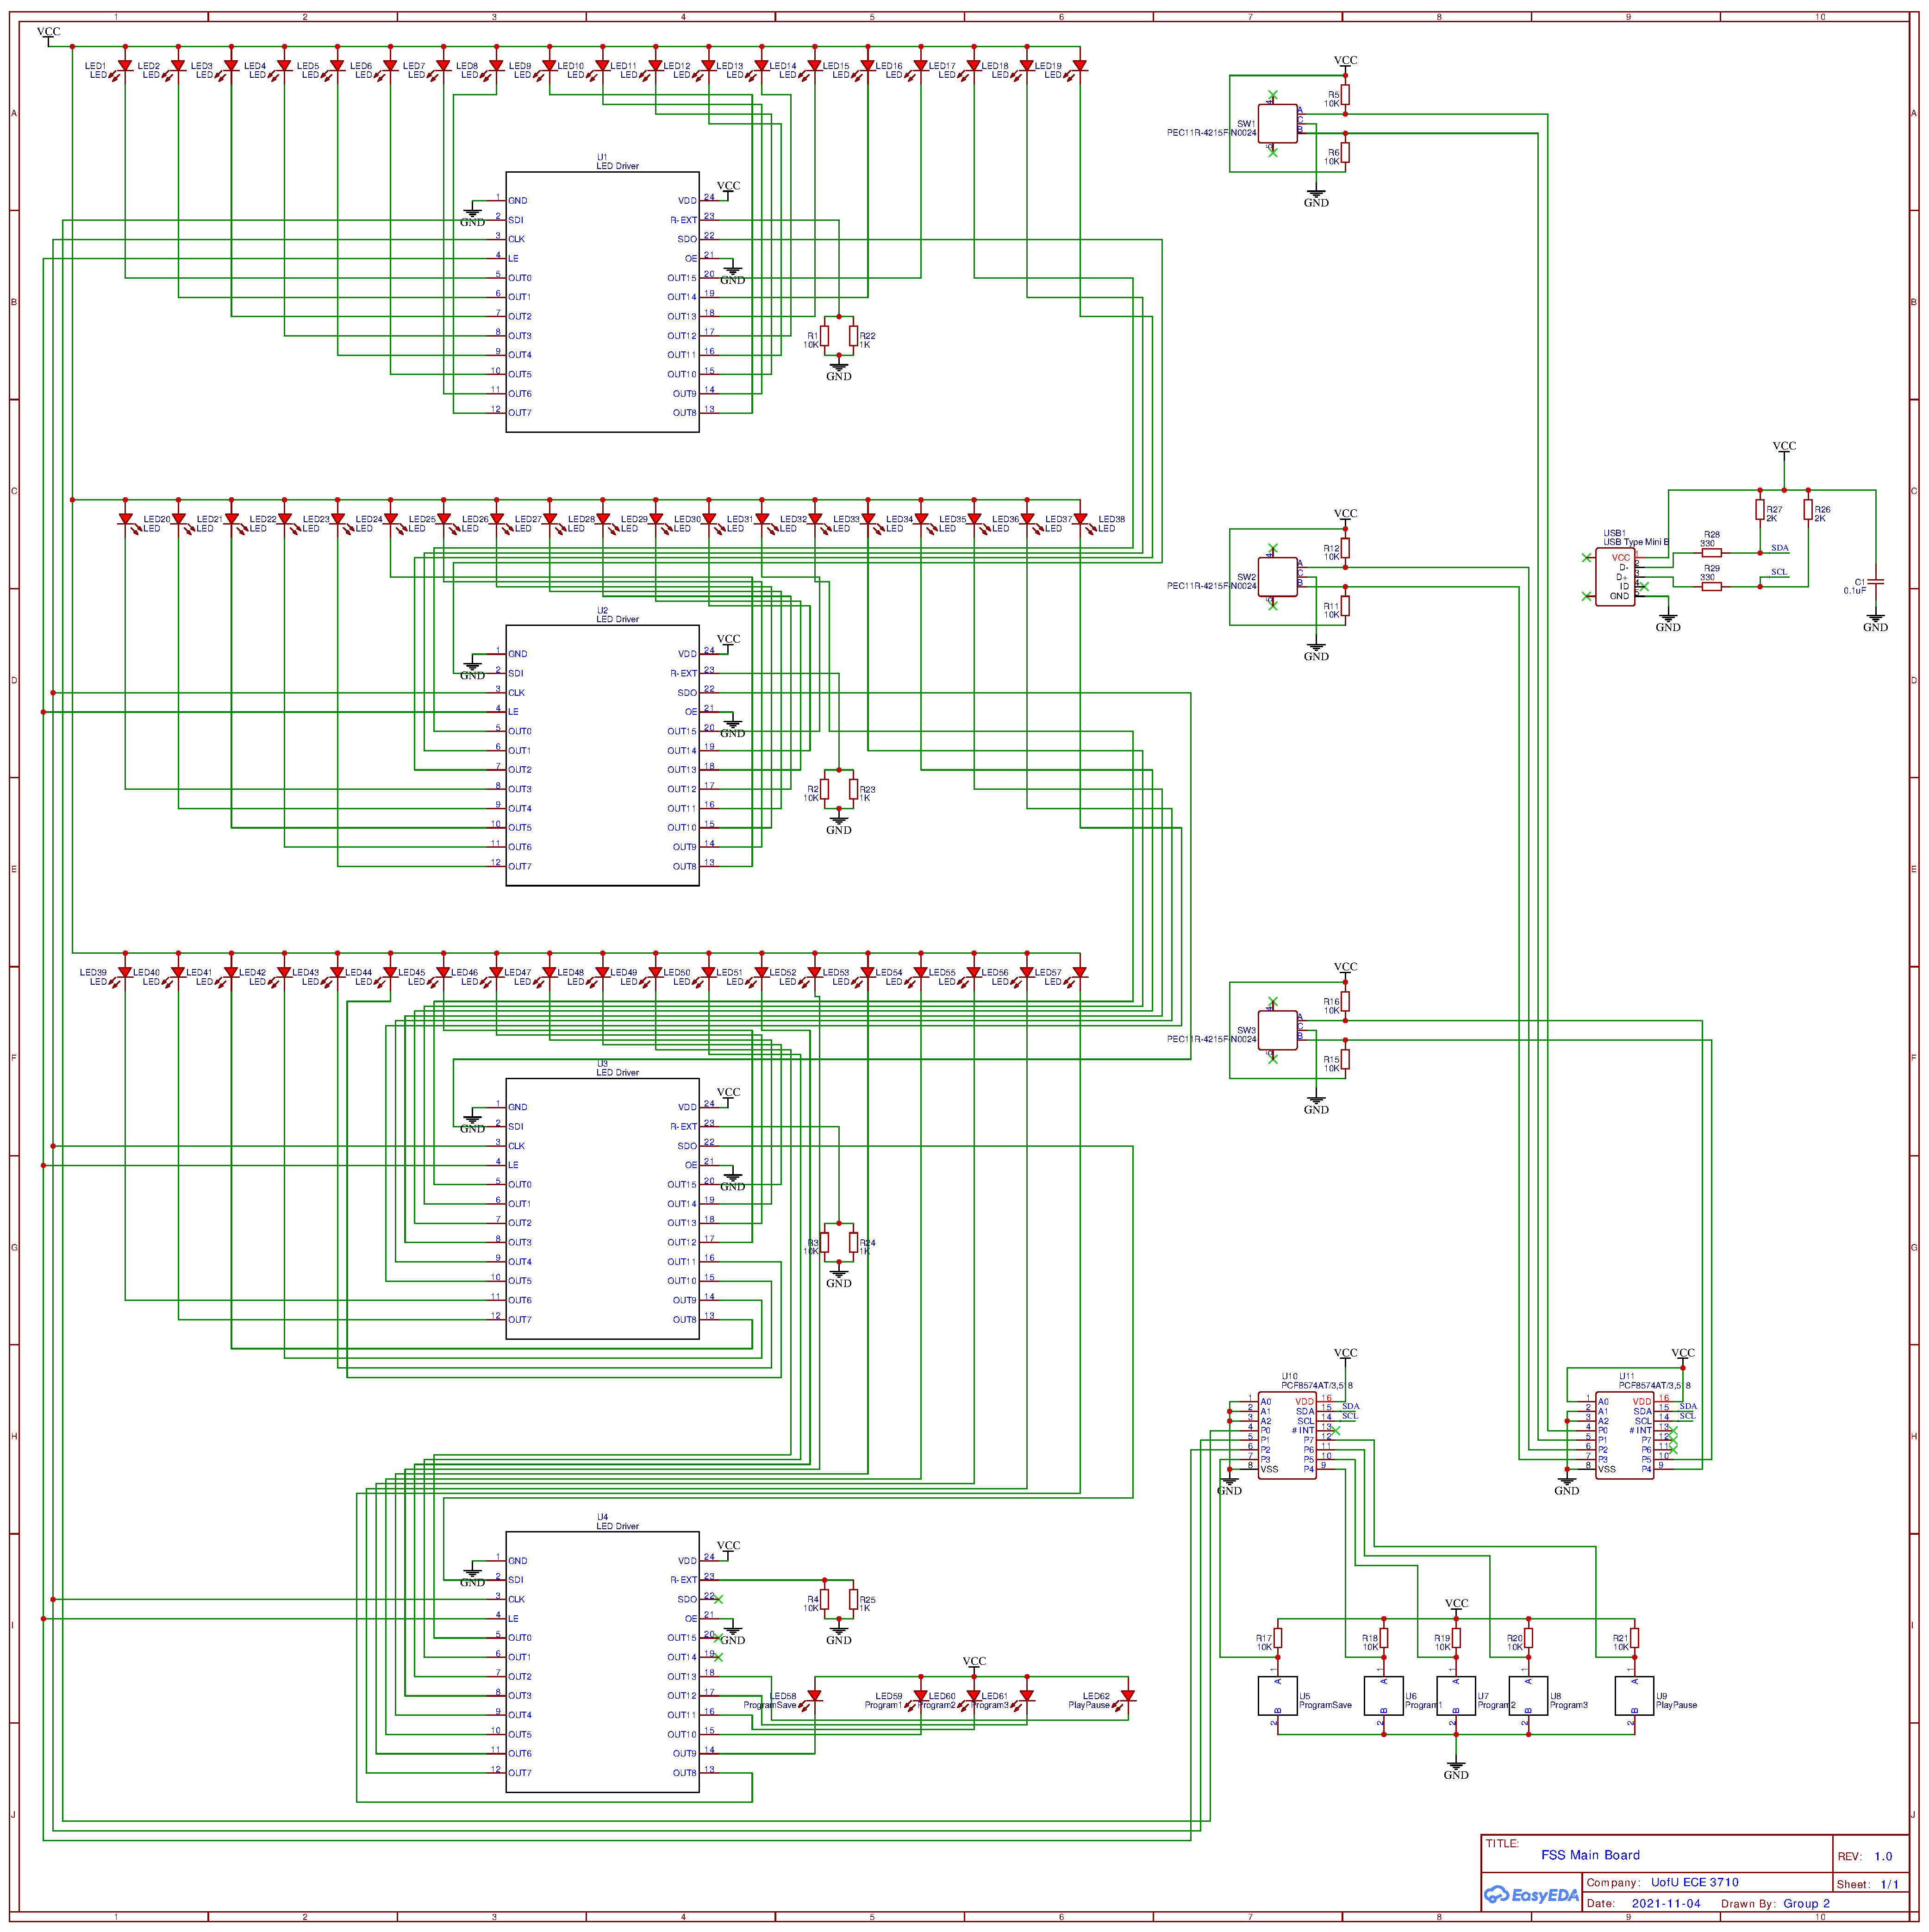
\includegraphics[width=6in]{./resources/figures/main_schematic.pdf}
    \caption{Schematic of main PCB.}
    \label{fig:main_schematic}
\end{figure*}

\begin{figure*}[bhtp]
    \centering
    \includegraphics[width=5.5in]{./resources/figures/main_pcb.pdf}
    \caption{Layout of main PCB.}
    \label{fig:main_pcb}
\end{figure*}

\begin{figure*}[bhtp]
    \centering
    \includegraphics[width=5in]{./resources/figures/main_pcb_assembly.jpg}
    \caption{Picture of main PCB assembly.}
    \label{fig:main_pcb_assembly}
\end{figure*}

\subsection{FSS Housing}
For the external housing, our team decided to go with a minimal design. The final assembly was constructed from stacked layers of acrylic panels, providing a solid structure with pleasing weight. The top layer was a sheet of translucent black acrylic, which allowed for our LED to shine through in a low amber color. Veneer surrounds the perimeter of the housing, giving a more natural feeling to the box. Finally, the knobs and control buttons were constructed out of acrylic to give them that same weight and sleek feeling the rest of the synthesizer gives. This design is minimal, but gives the user a sense a quality. By following a design process that takes the user's needs into account we were able to implement a device that is equal in both form and function. The final result has the quality and professional feeling that is geared toward musicians and producers.

The internals of the FSS housing can be seen in Figure 8. This picture is of an older version where we had used wood for the internal layers, before we replaced them with acrylic.

\begin{figure*}[bhtp]
    \centering
    \includegraphics[width=5in]{./resources/figures/housing_v1_back.jpg}
    \caption{Picture of FSS housing backside.}
    \label{fig:fss_walnut_front}
\end{figure*}

\section{CR16 Processor}
The details of our CR16 processor are contained in the previous lab reports, but for the purposes of the FSS Interface firmware, it would be enlightening to review some of the aspects of our CR16 ISA that were implemented specifically to abstract some useful functionality for the FSS Prototype. Although the processor we designed is mostly equipped for RISC instructions, these added instructions may have more of a CISC feel to them. The FSM controller of the CR16 CPU manages the fetch-decode-execute procedure for these instructions in the same way as the other instructions. Most of these instructions could be replaced by a series of RISC instructions, but we saved clock cycles by abstracting their behavior into the CPU FSM. Each of the following instructions is accompanied by an explanation for their implementation:
\begin{enumerate}
    \item \verb|LOADX/STOREX|: These instructions are external \verb|LOAD| and \verb|STORE| instructions which will be capable of storing data directly into an external memory address. This was implemented for two reasons. We want \verb|LOAD| and \verb|STORE| to have access to the whole address space of instantiated BRAM, and we want to be able to communicate in a modular way with GPIO registers that are sending and receiving information from the FSS GPIO port expanders over I$^2$C. These instructions also allow us to read a value from the microsecond counter, which is a separate Verilog module we created to assist with timing. Details on this module are explained in ``Peripheral Interfacing''.
    \item \verb|CALL/CALLD/RET| \textit{instead of} \verb|JAL/JUC|: Our software is quite long, and, for ease of development, we planned to use the stack to manage subroutine calls within subroutine calls. It seems to make more logical sense to encapsulate the management of the return address within the instruction. The \verb|CALL| and \verb|CALLD| (\verb|CALL| with displacement) instructions manage the return address implicitly, and \verb|RET| will be an unconditional jump to the previously calculated return address. This way, we don't need a dedicated register for the return address of a subroutine call.
    \item \verb|PUSH/POP|: These instructions encapsulate the behavior of modifying the stack pointer and loading/storing data in the stack. In order for them to work properly, the first instructions of any *.dat file to be run on the CR16 processor must assign an address to the stack pointer. By convention, we use the stack from the bottom of the file, i. e. address 1023 for a 10-bit address space. The stack ``lives'' in the same file as the code, so its capacity is between the EOF and the final machine-encoded instruction. Our processor has no kernel, and therefore has no notion of segmentation faults, so stack overflow has unintended and sometimes sneaky consequences.
\end{enumerate}

 The full ISA is located in the Appendix. This ISA may seem strange and unconventional, and it is likely less optimal than most standard accepted ISAs that fall cleanly into CISC or RISC categories. However, by the process of formulating our ISA, we have learned much about the considerations computer architects must make when designing an ISA. Our final CR16 ISA was assembled with a lot of careful thought and effort. The assembly software was a burdensome aspect of our project, so we are glad we had these features to develop it intuitively and cleanly.

\section{Peripheral Interfacing}
There are two peripherals that our FSS Prototype's firmware communicates with using the \code{LOADX/STOREX} instructions: the I$^2$C bus and a microsecond counter. The I$^2$C bus simply consists of two open-drain I/O pins --- one for SCL and one for SDA. These ports use the \code{inout} port direction in SystemVerilog to designate them as being used as both an input and an output. To create the open-drain configuration for these pins, the following Verilog code is used:
\begin{verbatim}
assign O_SCL = I_SCL_T ? 1'bZ : 1'b0;
assign O_SDA = I_SDA_T ? 1'bZ : 1'b0;
\end{verbatim}
This essentially creates two ground-driven, tri-state buffers with inverted triggers.

The microsecond counter is simply a clock divider in conjunction with 32-bit counter. Knowing that our CR16 processor clock uses our FPGA board's $50$ MHz clock, we can divide that by $50$ to create a clock signal with a period of 1 microsecond. Then with every pulse of the divided clock signal, a counter increments by 1.

These two peripherals are SystemVerilog modules that are instantiated in a another SystemVerilog module entitled \code{ext_mem}. This module maps addresses from the CR16 external memory port to the various external peripheral instantiations, namely: \code{clock_divided_counter} and \code{i2c_bus}. When the \code{LOADX/STOREX} instructions are decoded in the CR16 processor, the external memory port addresses into the peripheral instantiations accordingly so that 16-bit values can be read or written to directly from our assembly code. This is very similar to how memory-mapped I/O is done in commercial-grade microcontrollers and SoCs.

\section{Assembler}
Our CR16 processor project includes an accompanying custom-built assembler to compile assembly code written in our specialized ISA. The assembler itself is written in Java and uses the Gradle build tool for dependency management and distribution building. A library entitled ``JCommander'' is used to handle command-line argument parsing seamlessly. Listing \ref{listing:assembler_command_line} command-line usage of our assembler is as follows:
\begin{figure*}
  \begin{lstlisting}
  Usage: assembler [options] <assembly code file path>
  Options:
    -d, --debug
      Turns on debug mode.
      Default: false
    -p, --max-padding-line
      The line number to which padding lines should be added to an output
      binary.
      Default: 0
    -v, --max-padding-line-value
      The decimal value of the padding lines.
      Default: 0
    -b, --number-base
      The number base of the output binary.
      Default: HEX
      Possible Values: [BINARY, DECIMAL, HEX]
    -o, --output
      The output binary file path. Defaults to <input assembly file>.dat.
    -s, --output-processed
      True to write the processed assembly to <output binary file
      path>.processed.asm.
      Default: false
  \end{lstlisting}
  \caption{Command-line usage of CR16 Assembler.}
  \label{listing:assembler_command_line}
\end{figure*}

When run, the input file is read into memory and the code lines is sanitized, meaning that all code comments and unnecessary whitespace are removed. Comments in our assembly syntax are delimited using the hashtag symbol (e.g. ``\#''). Then macros are indexed and processed. A macro is used to create a mapping between a string (the key) and another string (the value). The following shows an example of how a macro is used in our firmware's assembly code to define the upper and lower 8-bits of the stack pointer:
\begin{verbatim}
# Initialize the stack pointer at BRAM
# address 0x0FFF (which is 2^12 - 1)
`define STACK_PTR_LOWER 0xFF
`define STACK_PTR_UPPER 0x0F
\end{verbatim}
Macros are used in several places in our firmware's assembly code as they are primarily used to give names to numerical constants.

Once macros have been processed, labels are then indexed and processed. Labels are used to reference static memory addresses, which allows a programmer to declare named functions and define static memory block. Listing \ref{listing:assembly_code_labels} following shows an example of how labels are used in our firmware's assembly code. This example listing contains an \code{.array_copy} function implementation that's prepended with our ``AssemblyDoc'' documentation. Note that the assembler will compile the \code{JLO .array_copy:loop} line to a branch instruction since the \code{.array_copy:loop} label is within the branch instruction's displacement range (which is $\pm127$). Similarly, a \code{CALL} instruction will compile to a \code{CALLD} instruction in the event that the given label is within the \code{CALLD} instruction's displacement range (which is $\pm2048$). Also note that if a programmer uses a \code{CALL} or jump instruction and the desired label to call/jump to is outside the displacement range of the equivalent displacement instruction, then the assembler will force the programmer to use an ``address loading register'' with the following syntax: \verb|JLO .far_away_label$r0|. This forces the programmer to make a conscience decision about which register the label address should be loaded into via the \code{MOVIL} (move-immediate lower 8-bits) and \code{MOVIU} (move-immediate upper 8-bits) instructions.
\begin{figure*}
  \begin{lstlisting}
##
# Copies the array at 'r11' to 'r12' with length 'r13'.
#
# @param r11 - a pointer to the array to copy from
# @param r12 - a pointer to the array to copy to
# @param r13 - the number of words to copy
#
# @return void
##
.array_copy
    MOVIL   r0  0x00
    MOVIU   r0  0x00

    .array_copy:loop

    LOAD    r5  r11
    STORE   r12  r5

    ADDI    r11 1
    ADDI    r12 1

    ADDI    r0  1
    CMP     r0  r13
    JLO     .array_copy:loop

    RET
  \end{lstlisting}
  \caption{The ``.array\_copy'' function from our firmware's assembly code.}
  \label{listing:assembly_code_labels}
\end{figure*}

Finally, the assembler will map all the instructions to their machine code equivalent as the CR16 ISA specifies. This machine code file is written according to the command-line arguments as shown in Listing \ref{listing:assembler_command_line}.

\section{Firmware}
The following discuss the functionality of our firmware's assembly code. We divided complex functions into smaller subroutines, allowing for the complexity of our firmware to be abstracted away piece-by-piece. This makes the assembly code much easier to read and is good programming practice.

\subsection{I\hspace{0.25mm}\texorpdfstring{$^{\textit{2}}$} CC Logic}
To interface with the I/O port expander chips via I$^2$C, a number of subroutines to handle writing and reading to and from the I$^2$C bus were programmed. Some simple ``getter'' and ``setter'' functions were created for the values of SDA and SCL lines. Then \code{START} and \code{STOP} conditions were programmed into separate functions to take control and release the bus respectively. A function for getting the acknowledge (ACK) bit from a slave and a function for sending the not-acknowledge (NACK) bit to a slave were also programmed. Lastly, functions for reading and writing arbitrary bits on the bus lines were programmed.

These simpler subroutines are called sequentially in the \code{.i2c_read_byte} and \code{.i2c_write_byte} functions. These function signatures are shown in Listings \ref{listing:assembly_i2c_read} and \ref{listing:assembly_i2c_write} respectively. The argument list gives a sense of how easily it is to read and write a byte to an addressable slave on the I$^2$C bus from anywhere in our firmware's assembly code. Note that in our setup, the FPGA board servers as the I$^2$C bus master and the I/O port expander ICs server as the slaves. More information on the I$^2$C protocol can be found \href{https://en.wikipedia.org/wiki/I\%C2\%B2C}{here}.
\begin{figure*}
  \begin{lstlisting}
##
# Requests to read a byte from a slave on the I2C bus.
#
# @param r11 - the 7-bit address of the I2C slave
#
# @return r10 - the byte read from the I2C bus or '0x0100' if a byte could not be read
##
.i2c_read_byte
  \end{lstlisting}
  \caption{The ``.i2c\_read\_byte'' function signature from our firmware's assembly code.}
  \label{listing:assembly_i2c_read}
\end{figure*}
\begin{figure*}
  \begin{lstlisting}
##
# Requests to write a byte to a slave on the I2C bus.
#
# @param r11 - the 7-bit address of the I2C slave
# @param r12 - the byte to write to the I2C slave
#
# @return r10 - 1 if successful, 0 if byte could not be written
##
.i2c_write_byte
  \end{lstlisting}
  \caption{The ``.i2c\_write\_byte'' function signature from our firmware's assembly code.}
  \label{listing:assembly_i2c_write}
\end{figure*}

\subsection{Microsecond Counter}
The microsecond counter module was added as a distinct Verilog module. The counter is 48 bits wide, and acts like a peripheral to the FSS device. We determined this to be a necessary bit width because $2^{32}$ microseconds is only about 71 minutes, and the software could misbehave if the counter ever resets. Since $2^{48}$ microseconds is about 8.9 years, the counter should never reset while the device is operating. Because the counter acts like a peripheral, its 48-bit count is stored in a set of 3 16-bit registers which can be accessed by encoded address using the \verb|LOADX| instruction. The counter module uses clock division logic with the 50MHz clock of the FPGA board to make an accurate count of the number of microseconds that have elapsed since the board was flashed with the synthesized hardware. One microsecond elapses after each 50 clock cycles from the 50MHz clock. When the microsecond counter data is fetched from the counter by assembly instructions, it can be used to take time stamps and calculate time elapsed. This is only feasible if the software can accommodate 48-bit unsigned subtraction. Thankfully unsigned subtraction and 2's complement subtraction are congruent. Therefore, we can use the \verb|SUB| instruction to subtract the least significant bits first, and then propagate any borrows to the next most significant bits. A borrow will never occur out of the MSB since the time elapsed will never reset to a lower number.

The most significant advantage of this functionality is that we could implement a helper function in the assembly which ``sleeps'' the hardware by a certain number of microseconds. This behavior is imperative to ensure correct protocol behavior with I$^2$C communication and LED animations.
\subsection{Rotary Encoder Polling}
The subroutine that receives the state of the three rotary encoders calls another subroutine for each rotary encoder to determine its spin direction. The encoder's spin direction determines how the ring LEDs should be lit on the next LED latch enable. Our chosen rotary encoders output a quadrature-encoded signal. Quadrature encoding is performed using two distinct bit values, where each value represents the state of a switch in the rotary encoder device. These values can be observed at terminals A and B as seen in Fig. \ref{fig:rotary_encoder_schematic}. From a high level, the spin direction can be determined by the appearance of the timing diagram for the two distinct signals. Fig. \ref{fig:quadrature_encoding} illustrates how a timing diagram may look when turning the rotary encoder in the clockwise direction, given that terminal A is the upper waveform and terminal B is the lower waveform.

\begin{figure}[h]
    \centering
    \includegraphics[scale=0.4]{./resources/figures/rotary_encoder_schematic.jpg}
    \caption{Schematic for PEC11R Series rotary encoders as seen in \cite{cite:rotary_encoders}}
    \label{fig:rotary_encoder_schematic}
\end{figure}

\begin{figure}[h]
    \centering
    \includegraphics[scale=0.4]{./resources/figures/quadrature_output_table.jpg}
    \caption{Waveform for a quadrature-encoded signal as seen in \cite{cite:rotary_encoders}}
    \label{fig:quadrature_encoding}
\end{figure}

The assembly code uses a static memory address in BRAM to store the previously obtained state of each rotary encoder, and the ``decode'' subroutine works to detect whether or not the rotary encoder has traversed a whole period of the quadrature output waveform. If it has, then the knob has been moved far enough to turn on or off an LED in the indicator ring.

\subsection{LED Animations}
One of our goals was to interface with the audio codec on our FPGA boards to generate sound, just as a commercial music synthesizer would, although, this goal was secondary. Due to time constraints, we instead implemented some very cool animations for the LEDs on the FSS Prototype. That includes a start up animation and 5 ``idle'' animation sequences. The pause/play button on the FSS was originally intended to pause and play the sound generated by the audio codec, but is now used to toggle between the various ``idle'' animation sequences. Some of these sequences pragmatically shift a number of 1's and 0's into the LED driver shift register with various delays. Other animation sequences use frame data located in static memory. These frames are encoded with the values (0 - 19) of the 3 ring displays and an animation function, entitled ``\verb|.execute_animation_sequence|'' steps through the frames with a 2 millisecond delay, decoding the frame and updating the LED driver shift registers accordingly.

\subsection{Business Logic and Final Device Integration}
With all of the sophisticated communication and data processing abstracted away, the business logic of the main routine actually becomes quite simple. On initialization, the FSS LED indicators light up with a brief startup animation. When the animation finishes, the FSS program loads program 1. The default program values are hard-coded into the firmware in a static location in memory which is referenced via a \code{.data} label. Because the FPGA must be reprogrammed every time it is turned off, we do not yet have a way to allow saved synthesizer programs to persist after shutdown, thus the saved program values only persist throughout program runtime. The firmware then enters into an infinite loop which integrates all the logic explained above to poll the state of the inputs from buttons and rotary encoders, process that data, and push the correct chain of 62 values onto the LED drivers. All of this occurs in a short time period, so no concurrency or event listening is necessary. The user receives practically instantaneous feedback to any stimulus applied to the dials or buttons.

Because we were too short on time to implement any audio functionality, we implemented some looping animations that will play when the user presses the play/pause button. These animations demonstrate the proper functioning of our I$^2$C communication, and some of them demonstrate the speed at which that communication can occur.

\section{Lessons Learned}
As a team, we feel that we have acquired many skills from the work we had to do for this project. Some of the most memorable lessons are learned when we make mistakes, and we would like to address a number of those lessons. These concepts apply to the software, electronics, and physical assembly aspects of our project, as well as our project management skills.

\begin{enumerate}
  \item Schematic Imperfections: Unfortunately, we to added a series resistor in the wrong place to our tactile push button and the rotary encoder channel pull-down configurations on our main PCB. Due to the fact that we were so concerned about accidentally shorting our I/O port expander chips, we placed resistors for short-circuit protection instead of resistors for normal operation. This issue was rectified easily by soldering series through-hole resistors to the push button and rotary encoder channel pull-down configurations.
  \item Common Ground: Unfortunately, we neglected one important detail about I$^2$C when we designed our breakout PCBs --- all masters and slaves on the bus need a common ground. The \code{GND} wire as shown in Figure \ref{fig:full_fss_block_diagram} was added after the PCBs were fabricated since the I$^2$C requirement of a common ground was neglected during the schematic development process. This issue was easily rectified by soldering a wire to the \code{OUT-} pin of the buck converter which could then be connected to the FPGA board's ground pin on the PMOD pin header.
  \item Rotary Encoder Filter Circuit: The datasheet for our rotary encoders contains a schematic for a suggested filter circuit, as seen in Fig. \ref{fig:rotary_encoder_schematic}. We neglected this circuit under the impression that the rest of our circuit would work to properly detect clean digital signals. During the hardware debugging process, however, we observe some noise around the channel transition thresholds, and we believe that a combination of the filter circuit and software debouncing would alleviate this issue.
  \item Water Jet Issues: Our first design was to utilize an anodized aluminum plate for the top surface of the device. We contracted a company here in the Salt Lake Valley to use a water jet to rout out the slots for the LED indicators and buttons. When we received the plates, there was evidence of a low-quality water jet job, with imprecise cuts and extremely rough edges. This was a disappointing waste of time, money, and materials. To combat this, we could have invested time in visiting the facility to view samples of the water jet work on anodized aluminum before committing to have them do our work.
  \item Wood is an Unreliable Material: Wood dimensions are not always as advertised depending on the climate and humidity of the supplier. In our particular application, wood panelling was too thin, and bowing made the assembly process unnecessarily difficult. Real wood veneer was also quite fragile, though the aesthetic was pleasing.
  \item Acrylic is an Expensive Material: To compensate for the challenges we faced with wood, we built the walls of the housing using layers of laser-cut acrylic sheets. This resulted in significant material waste, and was much more expensive than wood. In retrospect, something that could be 3D modelled and cast out of plastic would be much cheaper and more realistic for a preliminary prototype design, though the surface acrylic panelling was professional and sleek.
  \item Time Management: Many aspects of this project presented significant pressure for our group because of the ambitious nature of our project. We underestimated the amount of time we would spend testing, debugging, and correcting our CR16 processor and other software elements. As a rule of thumb, we should have doubled the time that we initially thought it would take to perform any task.
  \item Foam Buffers are not Good Support: The bottom panels make direct contact with foam buffers in the corners near the assembly screws, and this detracts from the rigidity of the rest of the design. The bottom plate can be pressed up into the rest of the device. To prevent this, the bottom plate should make direct contact with a rigid corner material and fit tightly.
\end{enumerate}
\section{Videos}
We wanted to create a professional video in the form of a product advertisement showing the beauty we captured in the FSS Prototype's design. That video is available \href{https://jacobpeterson.net/uofu-ece-3710/ad-video-redirect.html}{here}. Additionally, a demo video showing the basic usage and functional overview of the FSS Prototype is available \href{https://jacobpeterson.net/uofu-ece-3710/demo-video-redirect.html}{here}.

\section{About the Team}
There were many tasks involved in creating a functioning synthesizer, and due to this there was much overlap in the division of labor. To list a few:

\begin{itemize}
\item Concept Art
\item Assembly Programming
\item SystemVerilog Programming
\item Test Programs
\item Demo Programs
\item PCB Design
\item PCB Assembly and Reflow
\item Assembler
\item External Housing (Construction)
\item External Housing (Design)
\item Breakout Box Construction
\end{itemize}

Jacob and Nate covered much of the software, namely writing the FSS Prototype Verilog modules, the \code{fss.asm} assembly source code, creating demo programs, and implementing the core functionality of the synthesizer. They also worked together to physically assemble, reflow, and test the PCBs, and design the schematic for the breakout box PCB.

Jacob was also responsible for the peripheral interfacing --- writing the I$^2$C procedure in assembly --- and writing the assembler. He worked with Brady to design the Main FSS Board schematic.

Brady conceptualized the idea of a fully synchronized synthesizer and created all of the concept art. He also had a hand in creating test programs, designing the PCB, and designing and constructing the external housing. He and Jacob selected all of the device materials and acquired datasheets in their efforts to design the PCB and physical device housing.

Isabella assisted in creating test programs and constructing the external housing. She also created the synthesizer's breakout box and was responsible for modeling components in SolidWorks before 3D printing.

\section{Conclusion and Future Work}
Overall the final synthesizer came together well and the program reflects most our initial requirements. We were able to design and create a machine that properly updates parameters based on user inputs and can save those into memory to be loaded again when needed later. The final physical product is sleek, adequately reflects the current state of the program, and is simple to use.

In this version of our synthesizer we did not have time to tackle the audio codec on the FPGA. In a future implementation we hope to get this working so that our synthesizer may play music, and have the three dials correspond to audio settings that adjust the sound of the music playing. Beyond this, we would also like to add more inputs, than just the three simple dials. Other commercially available synthesizers have numerous knobs and switches that give users extensive control over the sound the synthesizer makes, and three knobs simply isn't enough to do this.

With these changes, our team could create a high quality synthesizer that has just as much form as function.

\begin{thebibliography}{10}

\bibitem{cite:github_compactrisc16}
  Github,
  Github Repository for ``CompactRISC16'',
  Fall 2021,
  \href{https://github.com/Petersoj/CompactRISC16}{Online}.

\bibitem{cite:github_fssprototype}
  Github,
  Github Repository for ``FSSPrototype'',
  Fall 2021,
  \href{https://github.com/Petersoj/FSSPrototype}{Online}.

\bibitem{cite:rotary_encoders}
  PEC11R Series 12mm Incremental Encoder,
  Bourns,
  PEC11R-4015F-N0024,
  \href{https://www.mouser.com/ProductDetail/Bourns/PEC11R-4015F-N0024?qs=Zq5ylnUbLm5obMMbrbYrpA\%3D\%3D}{Online}.

\bibitem{cite:de1-soc_manual}
  DE1-SoC User Manual,
  TerAsic Technologies,
  April 20216,
  \href{https://www.intel.com/content/dam/www/programmable/us/en/portal/dsn/42/doc-us-dsnbk-42-1004282204-de1-soc-user-manual.pdf}{Online}.

\end{thebibliography}

\clearpage
\setboolean{@twoside}{false}
\includepdf[pages=-, offset=0 0]{"../../../CompactRISC16/docs/Datasheets/CR16 ISA/CR16 ISA.pdf"}

\end{document}
